\section{Design of the Trunk Opening Control System}
\subsection{Specifications}
The system is fully synchronous, and all pulses last longer than the clock period.  
It has the following characteristics:

\underline{4 Inputs:}
\begin{itemize}
    \item 3 Push buttons ("BP0", "BP1", "BP2") used to enter a code.
    \item 1 Trunk lock input ("V") – when $V=1$, the trunk locks again.
    \begin{itemize}
        \item Note: This input has no effect if the trunk is not open.
    \end{itemize}
\end{itemize}

\underline{1 Output:}
\begin{itemize}
    \item 1 trunk opening signal ($S=1$ opens the trunk).
\end{itemize}

\underline{4 States:}
\begin{itemize}
    \item $E_0$: No button pressed.
    \item $E_1$: "BP0" pressed.
    \item $E_2$: "BP0 BP1" pressed.
    \item $E_3$: "BP0 BP1 BP2" pressed / Trunk opened.
\end{itemize}

\textbf{Important:} If two buttons are pressed simultaneously, the code entry resets (the system detects this as an error).  

\textbf{Note:} Due to a labeling mistake, the buttons are "BP0", "BP1", and "BP2" instead of "BP1", "BP2", and "BP3" as stated in the original specifications.

\subsection{State Diagram (Moore Machine Design)}
The following figure represents the system's state diagram:

\begin{figure}[H]
\centering
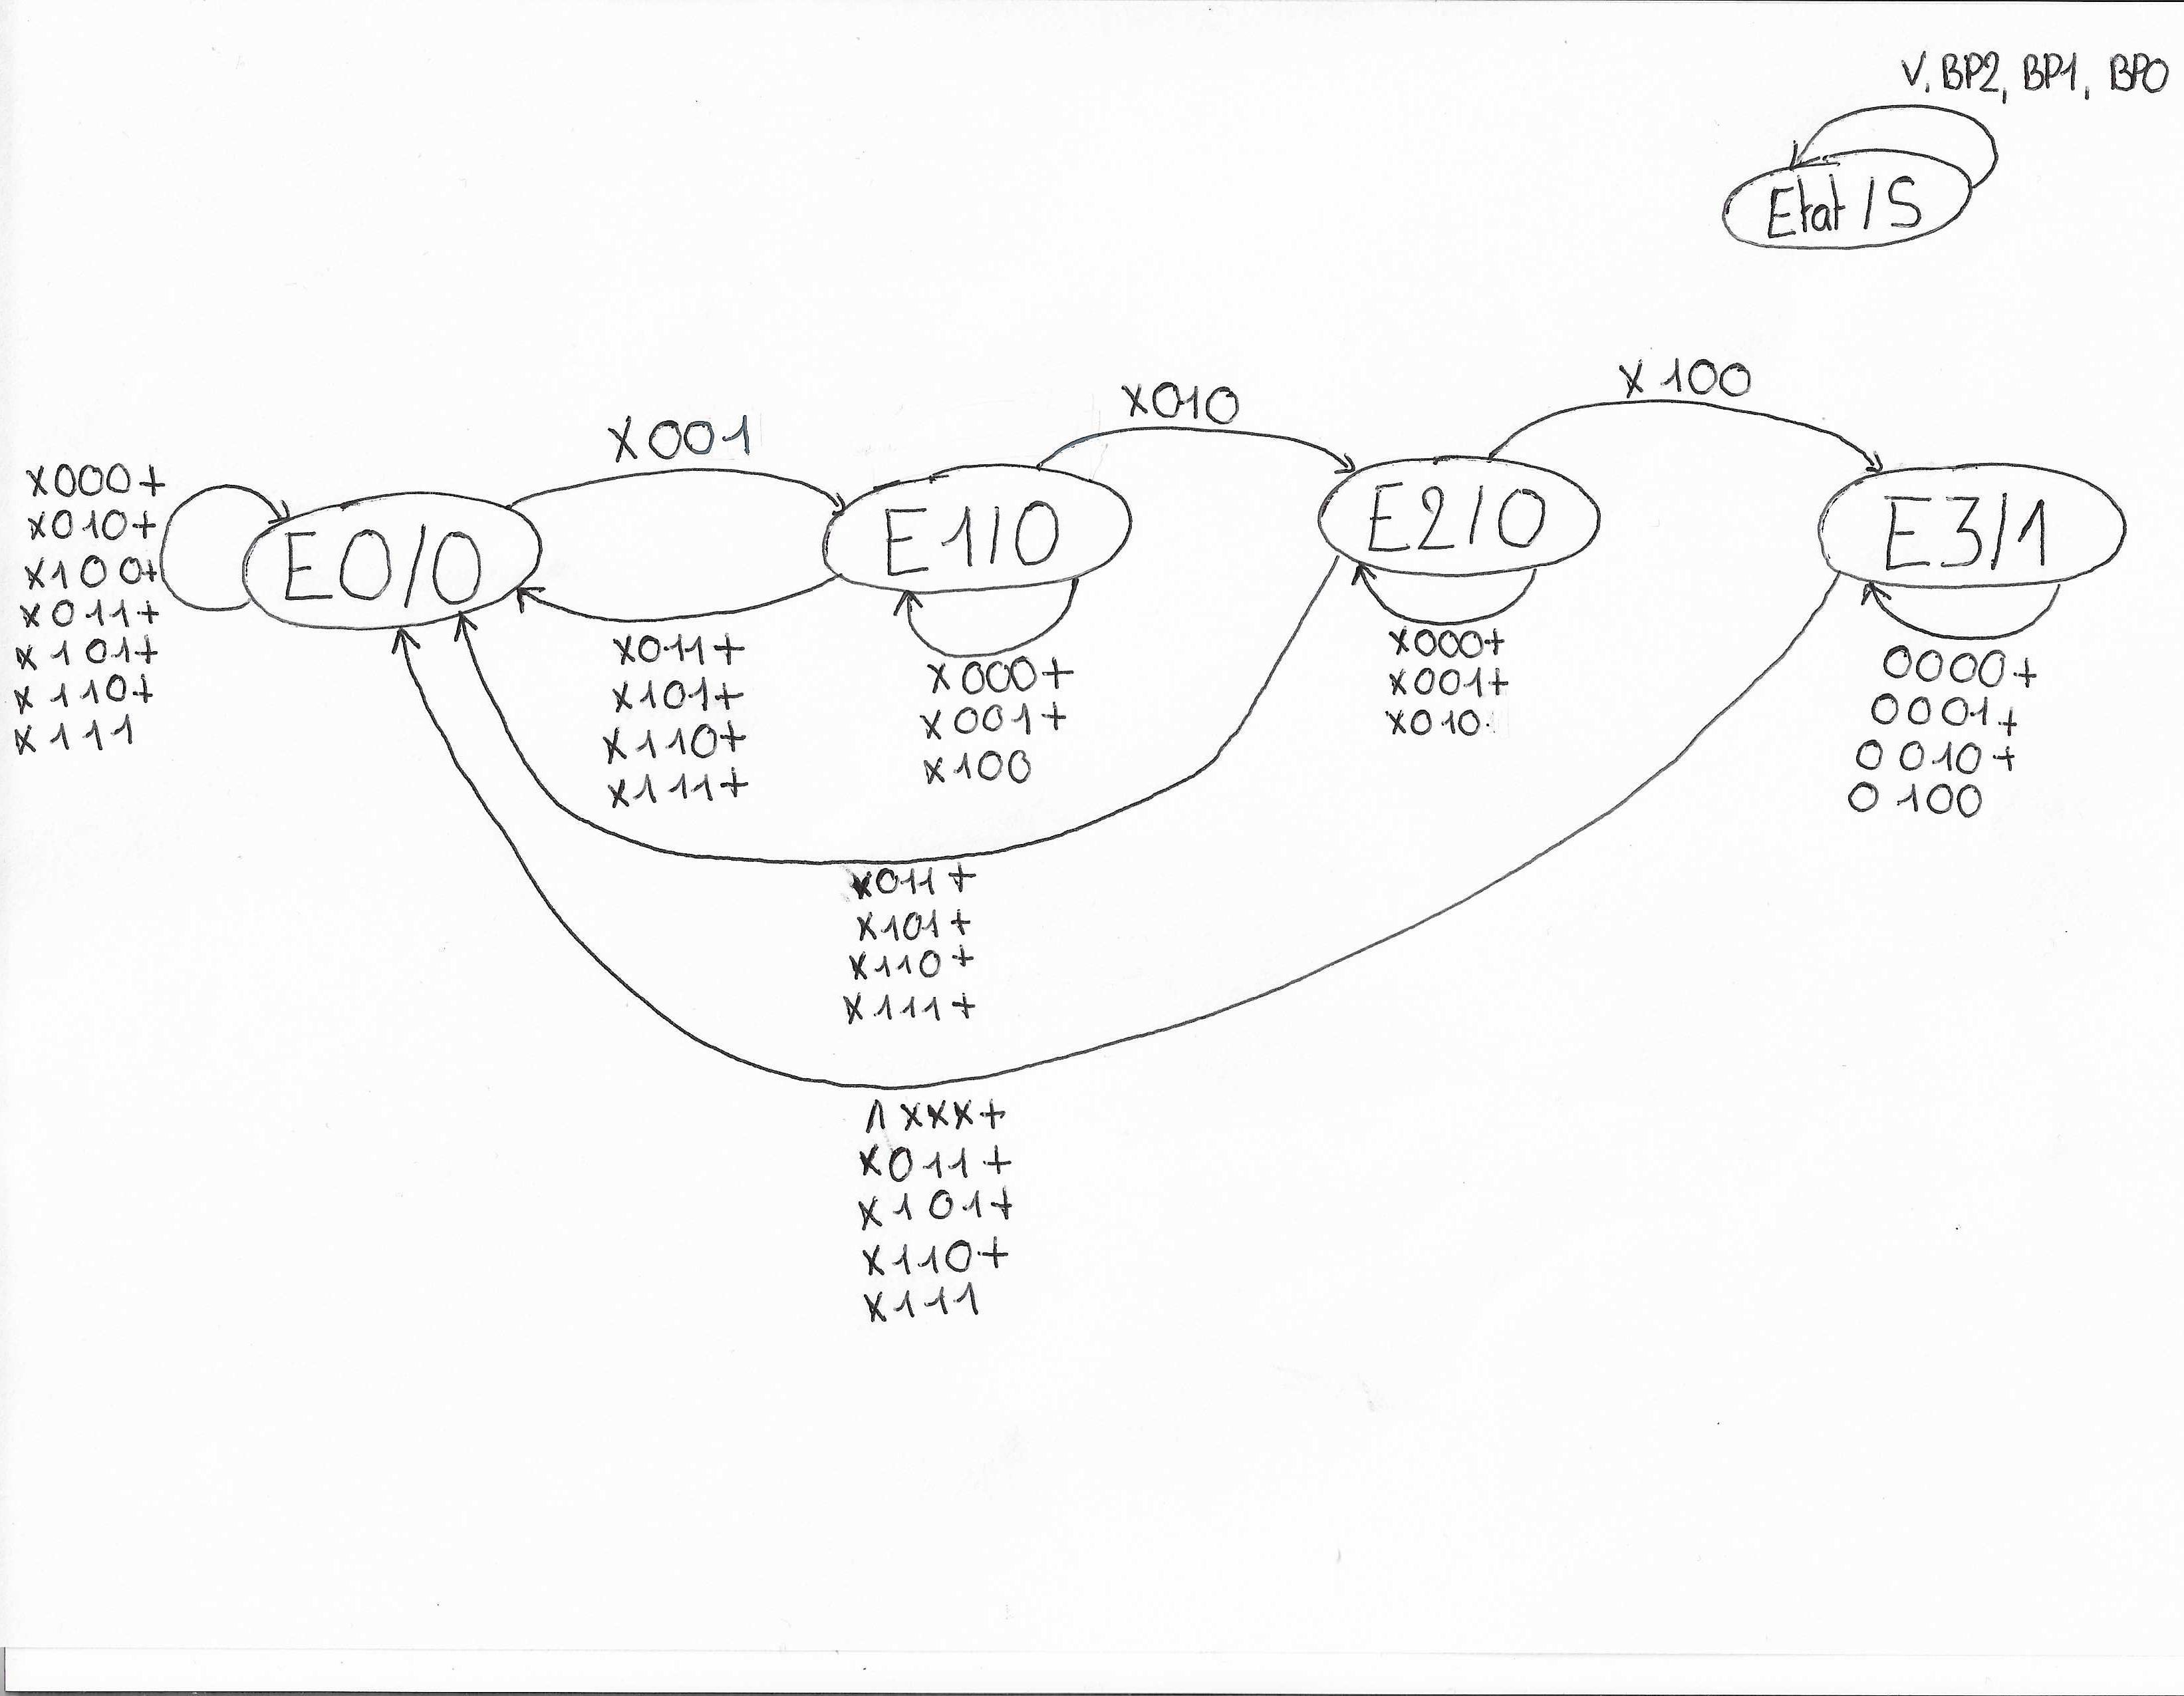
\includegraphics[height=10cm]{img/graph.jpg}
\caption{State diagram of the system}
\end{figure}

\newpage
\subsection{Deriving Flip-Flop Inputs and Output Expressions}
\subsubsection{State Transition Table}
From the previous state diagram, the following transition table is obtained:

\begin{figure}[H]
\centering
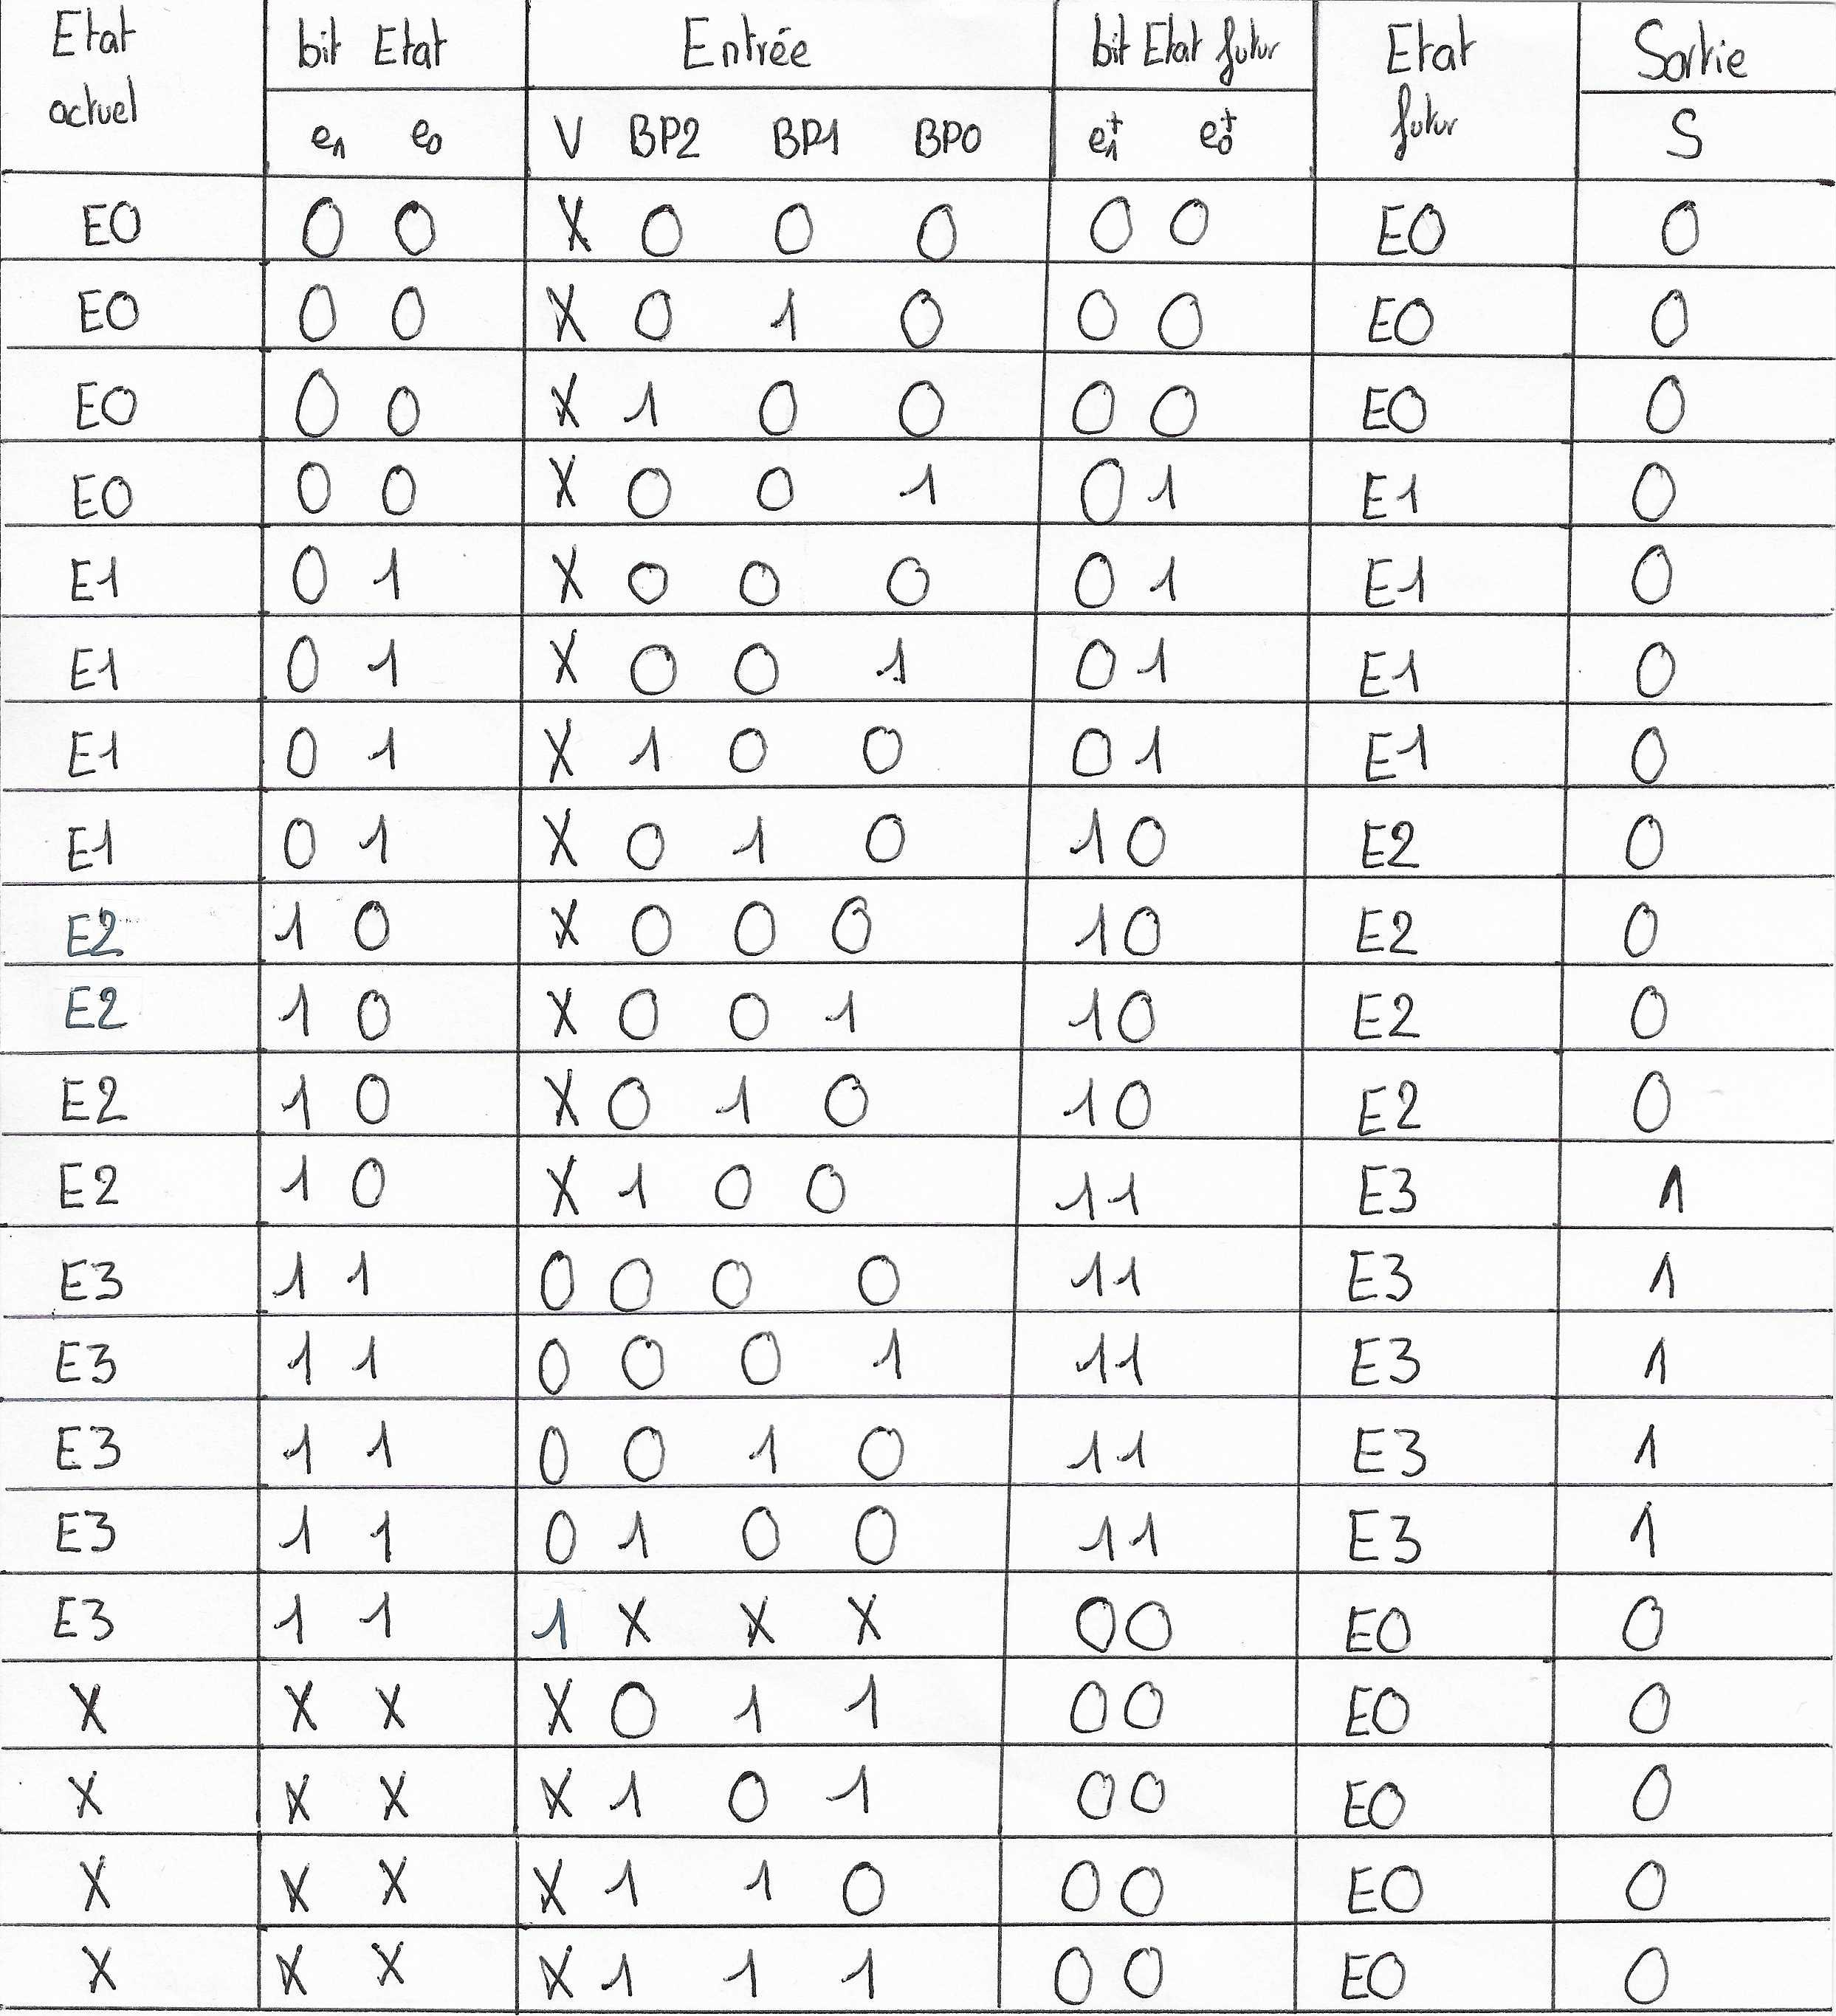
\includegraphics[height=10cm]{img/transition.jpg}
\caption{State transition table of the system}
\end{figure}

\newpage
\subsubsection{Karnaugh Maps}
\paragraph{Karnaugh Map for $e_0^+$}
Using the transition table, we derive the Karnaugh map for $e_0^+$:

\begin{figure}[H]
\centering
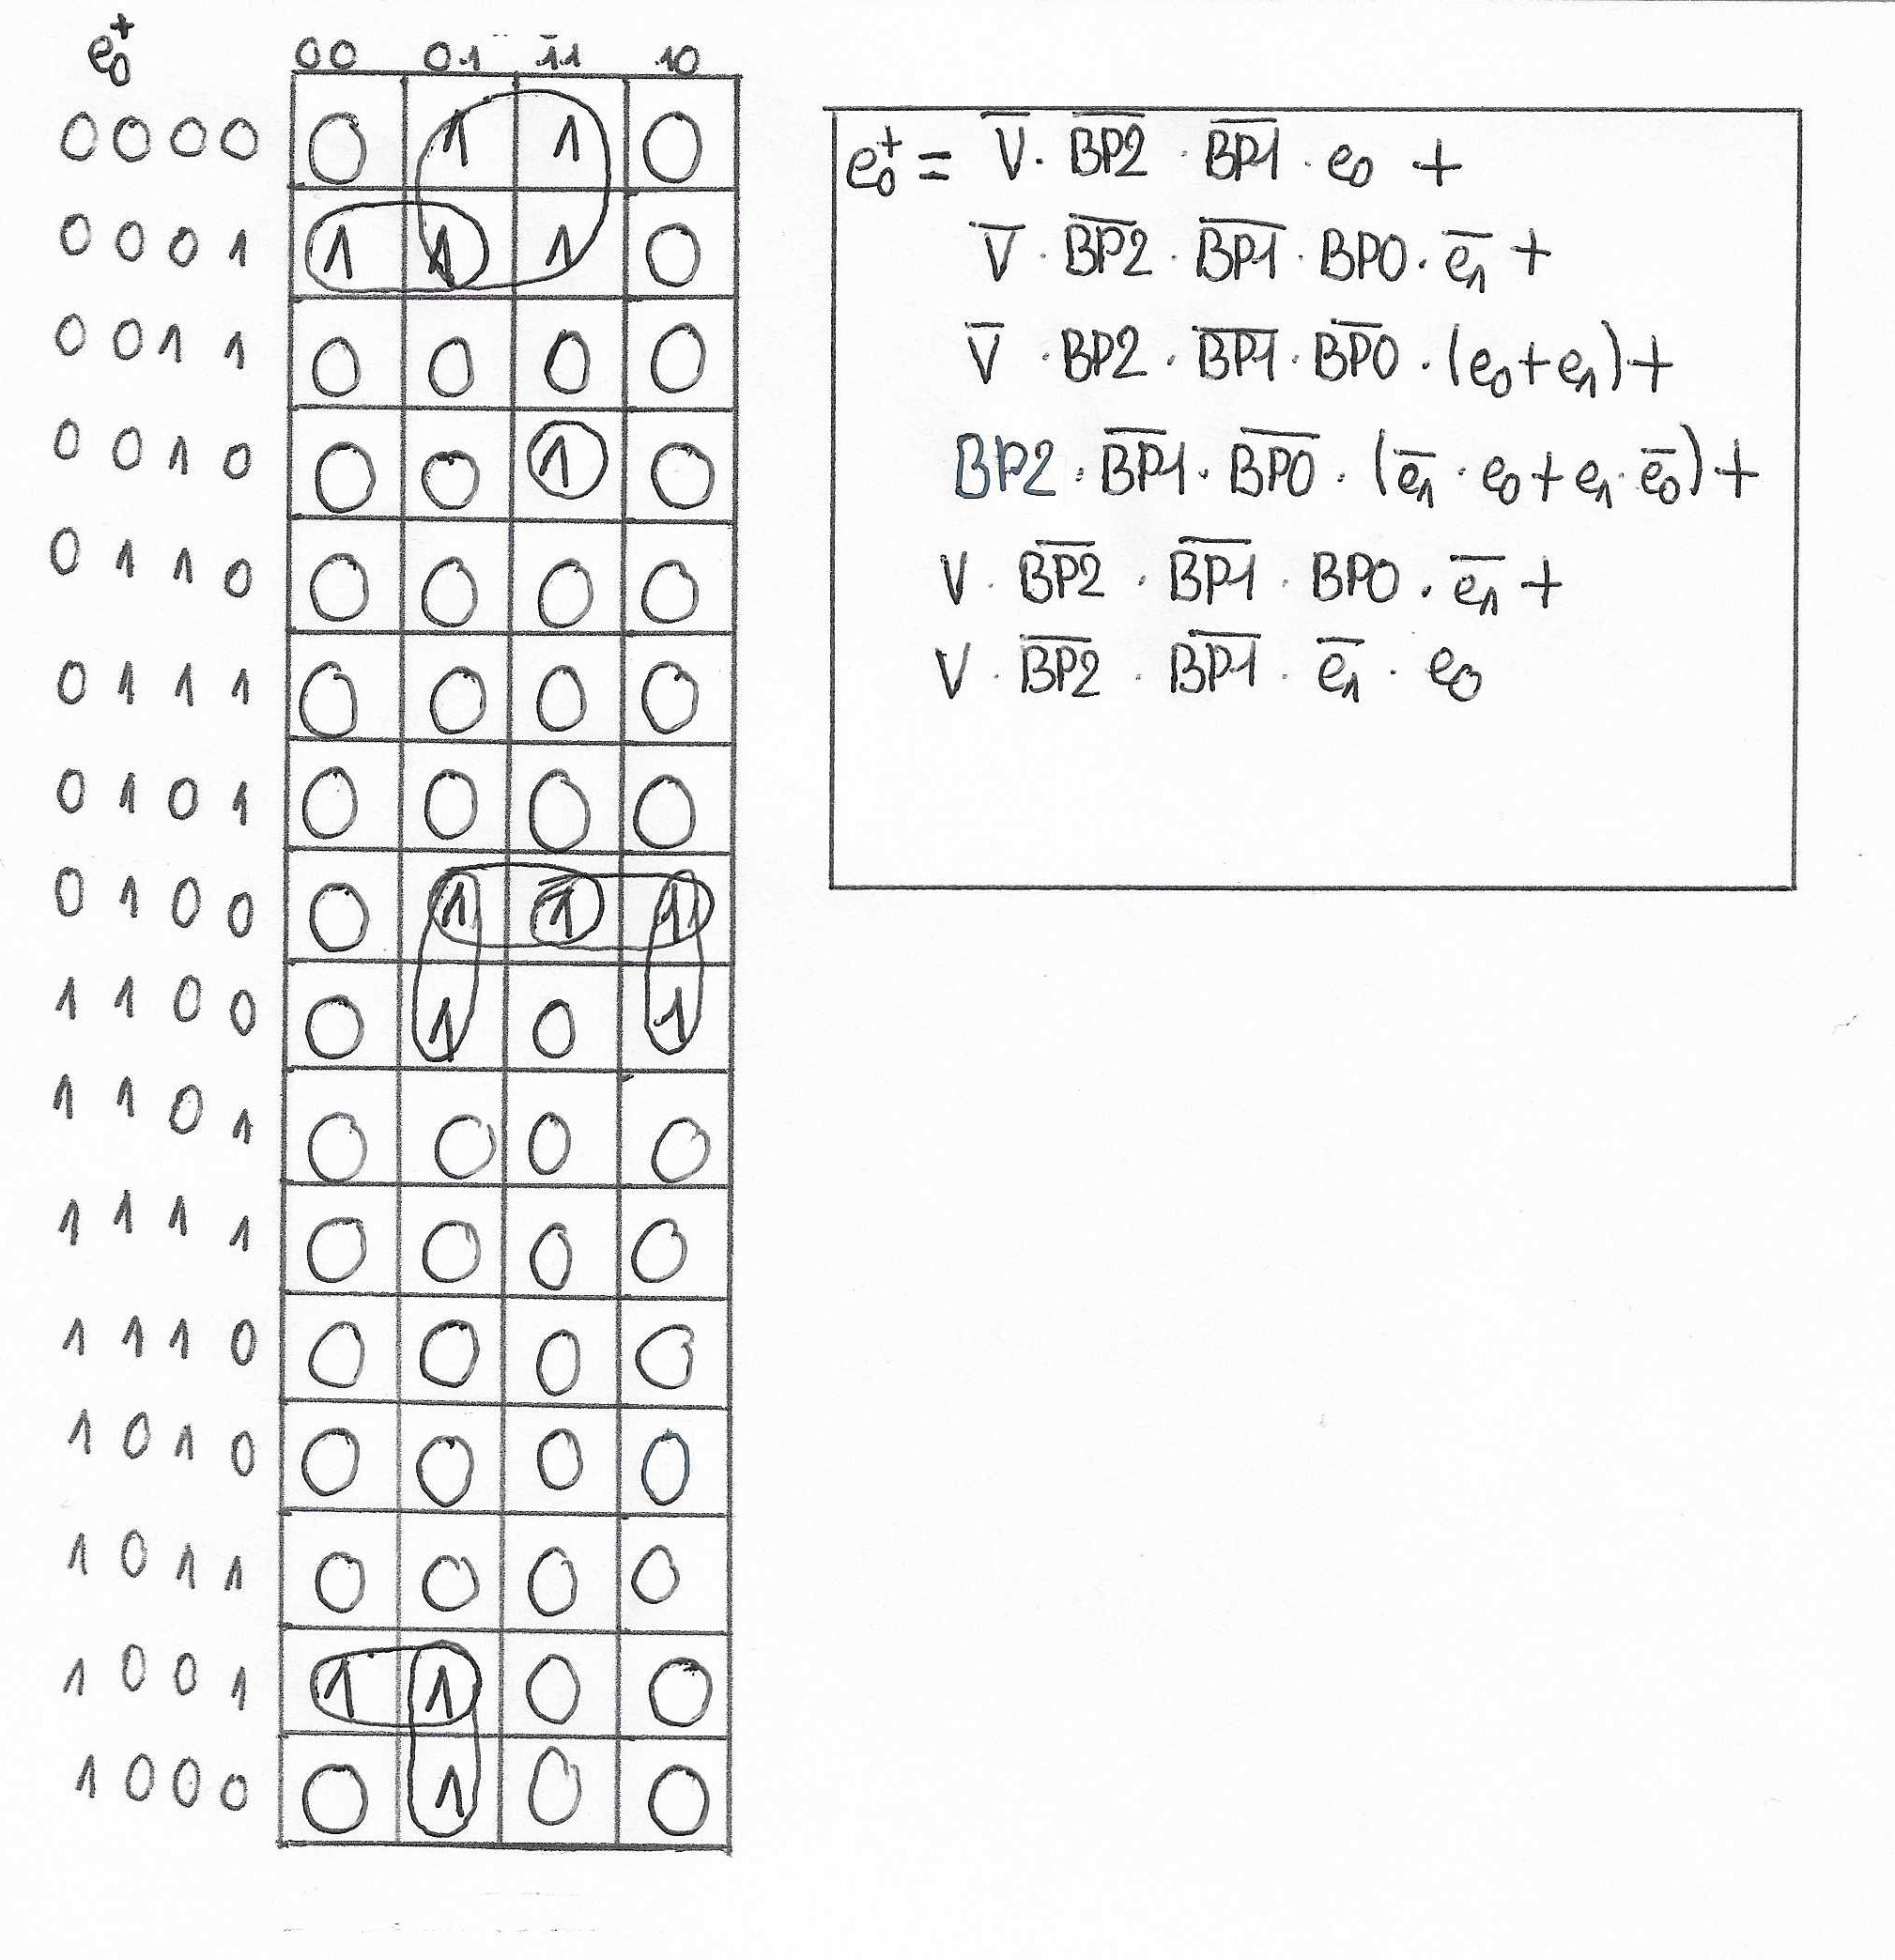
\includegraphics[height=9cm]{img/karnaugh_e0.jpg}
\caption{Karnaugh map for $e_0^+$}
\end{figure}

\paragraph{Karnaugh Map for $e_1^+$}
Using the transition table, we derive the Karnaugh map for $e_1^+$:

\begin{figure}[H]
\centering
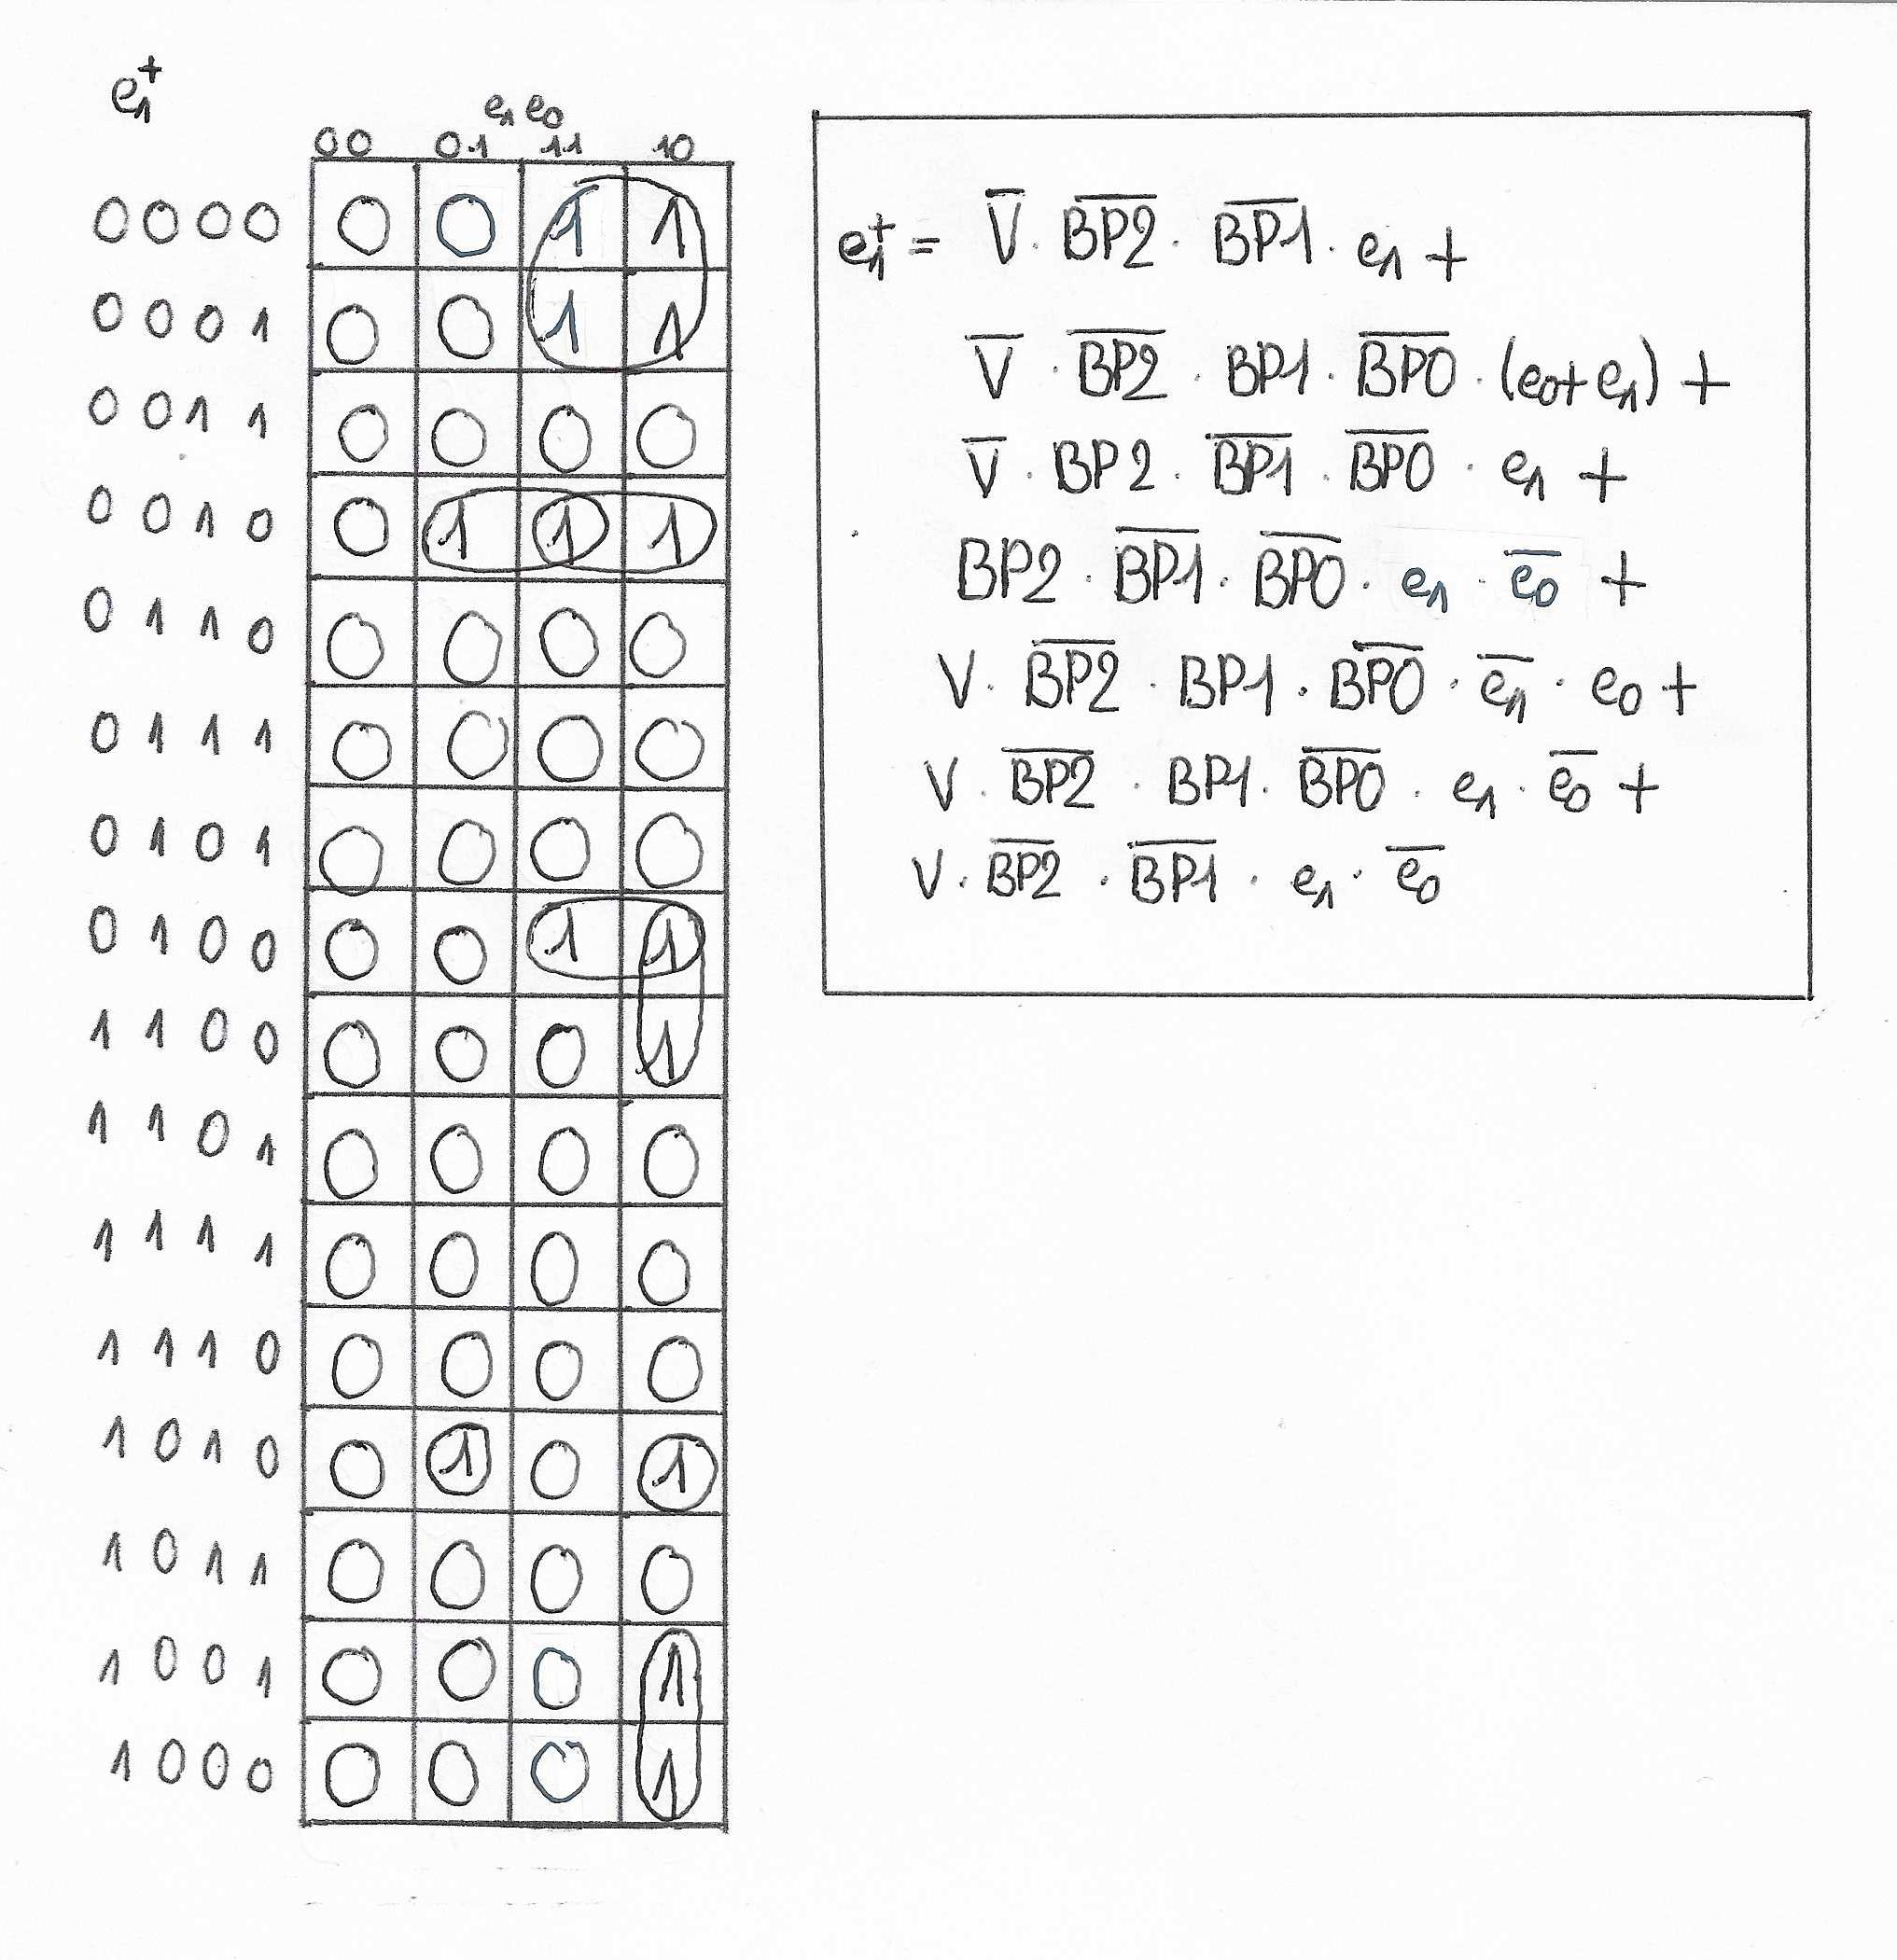
\includegraphics[height=9cm]{img/karnaugh_e1.jpg}
\caption{Karnaugh map for $e_1^+$}
\end{figure}

\paragraph{Output Expression Derivation}
From the transition table, the output equation is directly obtained as:  
\[ S = e_0 \cdot e_1 \]

\newpage
\subsection{System Design with D Flip-Flops}
Based on the previous equations, the following circuit is implemented:

\begin{figure}[H]
\centering
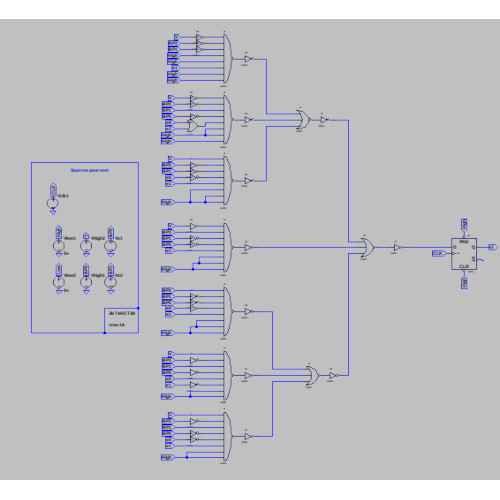
\includegraphics[height=7cm]{img/circuitE1.jpg}
\caption{Circuit section for generating $e_0$}
\end{figure}

\begin{figure}[H]
\centering
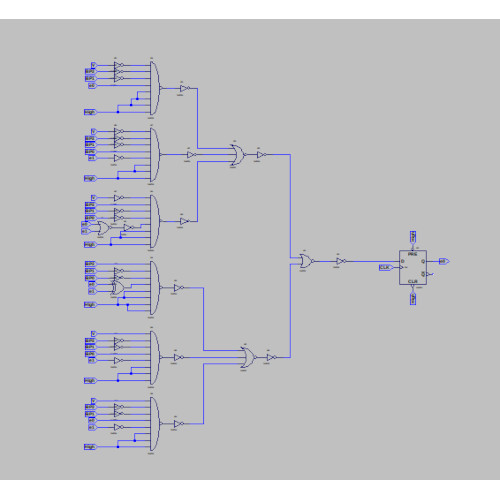
\includegraphics[height=7cm]{img/circuitE2.jpg}
\caption{Circuit section for generating $e_1$}
\end{figure}

\begin{figure}[H]
\centering
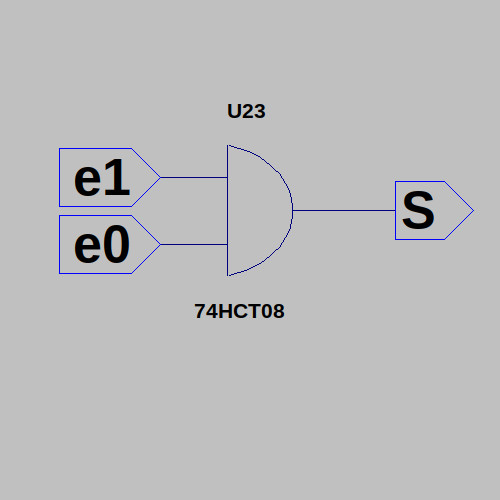
\includegraphics[height=5cm]{img/circuitS.jpg}
\caption{Circuit section for generating S}
\end{figure}

\newpage
\subsection{System Simulation and Testing in LTSpice}
To validate the circuit, a test scenario is created, leading to the following simulation:

\begin{figure}[H]
\centering
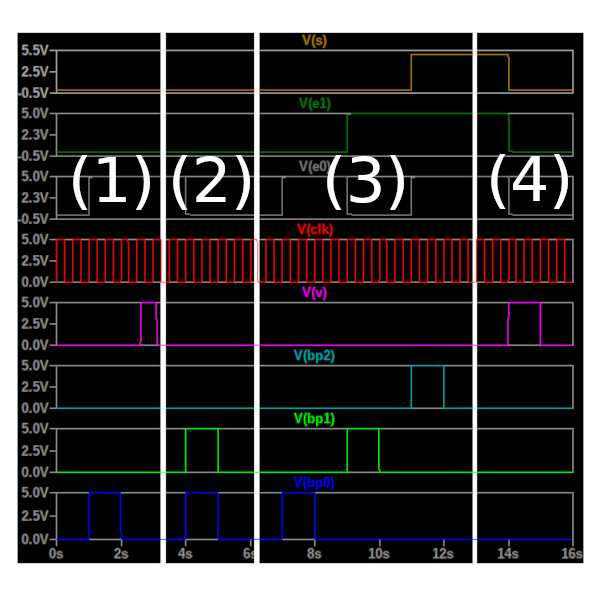
\includegraphics[height=9cm]{img/simu.jpg}
\caption{Circuit test using a simulated scenario}
\end{figure}

\textbf{Test Scenario (corresponding steps are labeled in the simulation):}
\begin{itemize}
    \item \textbf{Step 1:}  
    The operator presses "BP0", transitioning to $E_1$ ($e_1=0$, $e_1=1$).  
    Then, the operator presses "V" – nothing happens as expected, since "V" should have no effect unless the trunk is open.
    
    \item \textbf{Step 2:}  
    Still in $E_1$ ($e_1=0$, $e_1=1$). The operator presses "BP0" and "BP1" simultaneously, resetting the state to $E_0$ ($e_1=0$, $e_1=0$).  
    The system detects an error, requiring the code to be re-entered.
    
    \item \textbf{Step 3:}  
    \begin{itemize}
        \item The operator presses "BP0" → transitions to $E_1$ ($e_1=0$, $e_1=1$).
        \item The operator presses "BP1" → transitions to $E_2$ ($e_1=1$, $e_1=0$).
        \item The operator presses "BP2" → transitions to $E_3$ ($e_1=1$, $e_1=1$), and the trunk opens ($S=1$).
    \end{itemize}
    
    \item \textbf{Step 4:}  
    "V" is set to high, returning the system to $E_0$ ($e_1=0$, $e_1=0$), closing the trunk ($S=0$).
\end{itemize}
